\renewcommand{\FileId}{File: lab2.tex, Last changed: 2005-04-14}

%%%%%%%%%%%%%%%%%%%%%%%%%%%%%%%%%%%%%%%%%%%%%%%
% Switching Markov Loads and Rainflow Analysis
%%%%%%%%%%%%%%%%%%%%%%%%%%%%%%%%%%%%%%%%%%%%%%%

%\cleardoublepage
\chapter{Switching Markov Loads and Rainflow Analysis}
\label{lab2}

\section{Introduction}

In the PhD thesis ``Rainflow Analysis of Switching Markov Loads'',
Johannesson~\cite{Johannesson99.PhD} algorithms were developed for
calculating the theoretical rainflow matrix for switching processes,
and for decomposing a mixed rainflow matrix. (Some of the material
is also found in the Licentiate thesis ``Rainflow Cycles for Random
Loads with Markov Regime'', Johannesson~\cite{Johannesson97.Lic})
These algorithms were implemented in Matlab, and is included in the
WAFO toolbox.


%%%%%%%%%%%%%%%%%%%%%%%%%%%%%%%%%%%%%%%%%%%%%%%
% Markov Chains of Turning Points
%%%%%%%%%%%%%%%%%%%%%%%%%%%%%%%%%%%%%%%%%%%%%%%

\section{Markov Chains of Turning Points}

First we will examine a non-switching load, modelled as a Markov
chain of turning points.

%%%%%%%%%%%%%%%%%%%%%%%%%%%%%%%%%%%%%%%%%%%%%%%
% Model Definition and Simulation
%%%%%%%%%%%%%%%%%%%%%%%%%%%%%%%%%%%%%%%%%%%%%%%

\subsection{Model Definition}

The model is defined by the min-max matrix, \verb+G+. The matrix has dimension
$n \times n$, where $n$ is the number of discrete levels (e.g. $32$ or
$64$).
Here the discrete levels are chosen in the range
from $-1$ to $1$.
\begin{code}
>> n = 32; param = [-1 1 n];                % Define discretization
>> u = levels(param);                       % Discrete levels
>> G = mktestmat(param,[-0.2 0.2],0.15,1);  % min-max matrix
\end{code}
The command \verb+mktestmat+ (try \verb+help mktestmat+) creates a test matrix according to the
model in \cite[p.~127, Eqs.~(8.15,8.16)]{Johannesson99.PhD}.

%%%%%%%%%%%%%%%%%%%%%%%%%%%%%%%%%%%%%%%%%%%%%%%
% Simulation
%%%%%%%%%%%%%%%%%%%%%%%%%%%%%%%%%%%%%%%%%%%%%%%

\subsection{Simulation}

The model is easy to simulate and this is performed by the routine
\verb+mctpsim+
\begin{code}
>> T = 5000;                % Length of simulation (number of TP)
>> xD = mctpsim({G []},T);  % Simulate
>> x = u(xD)';              % Change scale to levels -1,..,1
\end{code}
and returns the discrete load \verb+xD+, which takes values
$1,\ldots,n$. By changing the scale of \verb+xD+ the load \verb+x+
takes values between $-1$ and 1. The first 200 samples of the
simulation is plotted by
\begin{code}
>> t=1:200; plot(t,x(t))
\end{code}


%%%%%%%%%%%%%%%%%%%%%%%%%%%%%%%%%%%%%%%%%%%%%%%
% Calculating the Rainflow Matrix
%%%%%%%%%%%%%%%%%%%%%%%%%%%%%%%%%%%%%%%%%%%%%%%

\subsection{Computation of the Limiting Rainflow Matrix}

% ADD: Definition of Grfc
The limiting rainflow matrix \verb+Grfc+ for the Markov model is
calculated by the routine \verb+mctp2rfm+.
\begin{code}
>> Grfc=mctp2rfm({G,[]});
\end{code}
A cycle matrix, e.g.\ a min-max or rainflow matrix, can be
plotted by \verb+cmatplot+.
Now we will compare the min-max and the rainflow matrices
\begin{code}
>> subplot(1,2,1),cmatplot(u,u,G),axis('square')
>> subplot(1,2,2),cmatplot(u,u,Grfc),axis('square')
\end{code}
Both 2D- and 3D-plots are possible draw,
see \verb+help cmatplot+. It is also possible to plot many matrices in
one call.
\begin{code}
>> cmatplot(u,u,{G Grfc},3)
\end{code}
Try also to plot with \verb+method=1+, which gives a 3D-plot, and
with \verb+method=4+, which gives contour lines.  Note that for high
maxima and low minima, the rainflow matrix has a pointed shape while
the min-max matrix has a more rounded shape.

Calculate the observed rainflow matrix obtained from the
simulation (using \verb|dtp2rfm|). Compare it with the theoretical one.
\begin{code}
>> FrfcObs = dtp2rfm(xD,n);
>> cmatplot(u,u,{FrfcObs Grfc*T/2})
\end{code}
In order to compare the observation \verb|FrfcObs| with the
theoretical rainflow matrix \verb|Grfc| we have to multiply it by the
number of cycles in the simulation which is equal to \verb|T/2|.

%%%%%%%%%%%%%%%%%%%%%%%%%%%%%%%%%%%%%%%%%%%%%%%
% Switching Markov Chains of Turning Points
%%%%%%%%%%%%%%%%%%%%%%%%%%%%%%%%%%%%%%%%%%%%%%%

\section{Switching Markov Chains of Turning Points}

%%%%%%%%%%%%%%%%%%%%%%%%%%%%%%%%%%%%%%%%%%%%%%%
% A Specified Model
%%%%%%%%%%%%%%%%%%%%%%%%%%%%%%%%%%%%%%%%%%%%%%%

%\section{A Specified Model}

Here we will examine an example of a switching load modelled by a
switching Markov chain of turning points. This is the same model as
used in \cite[p.~57, Example~4.1]{Johannesson99.PhD}. The load will
be a mixture of two subloads specified via its min-max matrices.
First we will define the model and make a simulation. Then we will
calculate the limiting rainflow matrix for the model and compare it
with a simple superposition of the two subloads and also with the
observed rainflow matrix from the simulation. Finally, we will
examine level crossings and damage.  See also the demo
\verb+rfcdemo2+ which considers the examples shown below of
switching Markov chains of turning points.

%%%%%%%%%%%%%%%%%%%%%%%%%%%%%%%%%%%%%%%%%%%%%%%
% Model Definition and Simulation
%%%%%%%%%%%%%%%%%%%%%%%%%%%%%%%%%%%%%%%%%%%%%%%

\subsection{Model Definition}

The model is defined by the min-max matrices
for each
subload together with the transition matrix \verb+P+ for the regime
process. Here we consider a mixture of two subloads, which are defined
according to model A in Table~\ref{TabMarkovTP:Templates}. (We will
examine model B later on.)
\begin{table}[htbp]
\begin{center}
\begin{tabular}{|c||r|r|r|r||r|r|r|r|}
  \hline
  & \multicolumn{4}{c||}{Model A} & \multicolumn{4}{c|}{Model B} \\ \hline
  subload $z$   & $x_{1z}$  & $x_{2z}$  & $s_z$  & $\lambda_z$
        & $x_{1z}$  & $x_{2z}$  & $s_z$  & $\lambda_z$ \\ \hline
  1     & -0.4      & -0.3      & 0.15   & 1.0
        &  -0.1      &  0.1      & 0.28   & 0.5 \\ \hline
  2     &  0.3      &  0.4      & 0.15   & 1.0
        & 0.0      &  0.0      & 0.12   & 2.0 \\ \hline
\end{tabular}
\end{center}
\caption{\emph{
    Parameters for the subloads of models A and B. The min-max matrix
    $\bm{G}$ for
    each subload is given by the templates describes
    in \cite[p.~127, Eqs.~(8.15,8.16)]{Johannesson99.PhD}. The subloads are
    assumed to be time-reversible, and hence the max-min matrix is
    $\bmh{G}=\bm{G}^T$.
    }}
\label{TabMarkovTP:Templates}
\end{table}
By using the routine \verb+mktestmat+, we specify the min-max
 matrices, \verb+G1+ and \verb+G2+. They both have dimension
$n \times n$, where $n=32$ is the number of discrete levels, ranging
from $-1$ to $1$.
\begin{code}
>> n=32; param = [-1 1 n];                   % Define discretization
>> u=levels(param);                          % Discrete levels
>> G1 = mktestmat(param,[-0.4 -0.3],0.15,1); % regime 1
>> G2 = mktestmat(param,[0.3 0.4],0.15,1);   % regime 2
\end{code}
Plot the matrices \verb+G1+ and \verb+G2+ by using \verb+cmatplot+.

Next we specify a transition matrix for the regime process. (You may
choose a different one if you like.)
\begin{equation} \label{EqMarkovTP:PmatrixA}
  \bm{P} = \left(
  \begin{array}{cc}
    0.90 & 0.10 \\
    0.05 & 0.95
  \end{array} \right)
\end{equation}
\begin{code}
>> p1=0.10; p2=0.05;
>> P=[1-p1 p1; p2 1-p2]                 % Transition matrix
>> statP=mc2stat(P)                     % Stationary distribution
\end{code}
which has stationary distribution \verb|statP|, equal to
$\bm{\rho}=(1/3,\, 2/3)$. This means that (in mean) $1/3$ of the time
is spent in regime 1 and $2/3$ of the time in regime 2.

%%%%%%%%%%%%%%%%%%%%%%%%%%%%%%%%%%%%%%%%%%%%%%%
% Simulation
%%%%%%%%%%%%%%%%%%%%%%%%%%%%%%%%%%%%%%%%%%%%%%%

\subsection{Simulation}

The model is simulated by the routine
\verb+smctpsim+
\begin{code}
>> T=5000;                      % Length of simulation (number of TP)
>> [xD,z] = smctpsim(P,{G1 []; G2 []},T); % Simulate
>> x=u(xD)';                    % Change scale to levels -1,..,1
\end{code}
and returns the switching load \verb+xD+, which takes values
$1,\ldots,n$, and the regime process \verb+z+. By changing the scale
of \verb+xD+ the switching load
\verb+x+ takes values between $-1$ and 1. The first 400 samples of the
simulation is plotted by
\begin{code}
>> t=1:400;
>> hmmplot(x(t),z(t),t,[1 2])         % Same colour
>> hmmplot(x(t),z(t),t,[1 2],'','',1) % Different colours
\end{code}
and a simulated load is shown in Figure~\ref{fig1:SamplePath}.
The regime process \verb+z+ controls the current characteristics of
the switching load \verb+x+, which is clearly seen as changes of the
mean level.
\begin{figure}[htbp]
  \centerline{
   \resizebox{\figwidthA}{\figheightA}{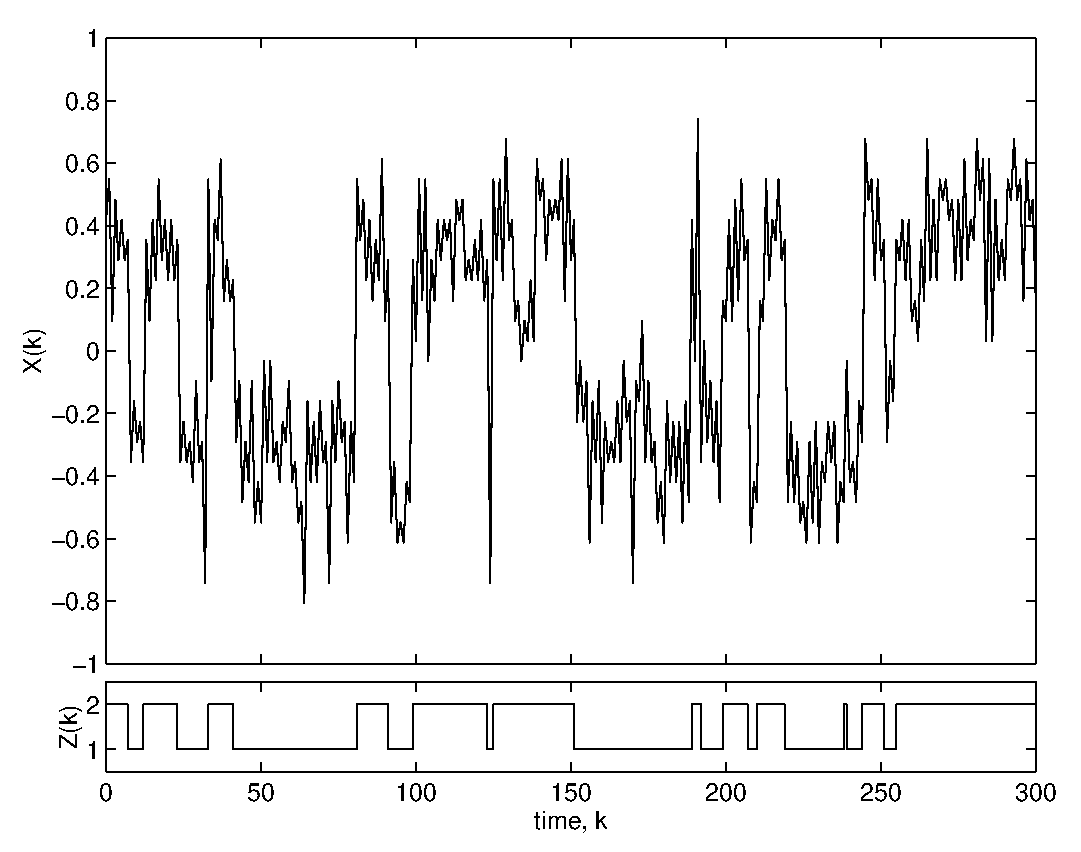
\includegraphics{fig/FigExTP1a_SamplePath.eps}}
  }
  \caption{\emph{The first 400 samples from a simulation of model A. The upper graph shows the turning points \emph{\texttt{x}} and the lower
    the regime process \emph{\texttt{z}}.}}
  \label{fig1:SamplePath}
\end{figure}


%%%%%%%%%%%%%%%%%%%%%%%%%%%%%%%%%%%%%%%%%%%%%%%
% Calculating the Rainflow Matrix
%%%%%%%%%%%%%%%%%%%%%%%%%%%%%%%%%%%%%%%%%%%%%%%

\subsection{Computing the Limiting Rainflow Matrix}

The two subloads are described by \verb+G1+ and \verb+G2+,
respectively, and their limiting rainflow matrices can be calculated
by the routine \verb+mctp2rfm+. The rainflow matrix for the
switching load is calculated by the routine \verb+smctp2rfm+ which
takes the transition matrix \verb+P+ together with \verb+G1+ and
\verb+G2+ as input.
\begin{code}
>> Grfc=smctp2rfm(P,{G1,[];G2,[]});
>> Grfc1=mctp2rfm({G1,[]});
>> Grfc2=mctp2rfm({G2,[]});
>> GrfcSum=statP(1)*Grfc1+statP(2)*Grfc2;
\end{code}
The matrix \verb+GrfcSum+ is a superposition of the rainflow
matrices for subloads 1 and 2, respectively. This is the rainflow
matrix we obtain if we don't take the switching into account. The
rainflow matrices can be plotted by \verb+cmatplot+.
\begin{code}
>> cmatplot(u,u,{Grfc1 Grfc2; GrfcSum Grfc})
\end{code}
%The calculated rainflow matrices for each regime \verb+Grfc1+,
%\verb+Grfc2+ and for the
%switching process \verb+Grfc+ are shown in
%Figure~\ref{fig1:rfc}a,b,c.
Note that, if
the  rainflow matrices for the two regimes are superimposed like
\verb+GrfcSum+, then the largest
cycles (low minima and large maxima) are lost, compare the two lower plots.
%Figure~\ref{fig1:rfc}c with~\ref{fig1:rfc}d.

%\begin{figure}[htbp]
%  \begin{tabular}{cc}
%    {\small (a) Rainflow matrix, \verb+Frfc1+}  &
%    {\small (b) Rainflow matrix, \verb+Frfc2+} \\
%    \resizebox{\figwidthB}{!}{\includegraphics{fig/Fig1rfc1.eps}} &
%    \resizebox{\figwidthB}{!}{\includegraphics{fig/Fig1rfc2.eps}} \\
%    {\small (c) Rainflow matrix, \verb+Frfc+}  &
%    {\small (d) Rainflow matrix, \verb+FrfcSum+} \\
%    \resizebox{\figwidthB}{!}{\includegraphics{fig/Fig1rfc.eps}} &
%    \resizebox{\figwidthB}{!}{\includegraphics{fig/Fig1rfcSum.eps}} \\
%  \end{tabular}
%  \caption{\emph{ 3D-plot of the rainflow
%      matrices
%      (a) regime 1,
%      (b) regime 2,
%      (c) switching process,
%      (d) weighted sum of regime 1 and 2.}}
%  \label{fig1:rfc}
%\end{figure}


%%%%%%%%%%%%%%%%%%%%%%%%%%%%%%%%%%%%%%%%%%%%%%%
% Model Definition and Simulation
%%%%%%%%%%%%%%%%%%%%%%%%%%%%%%%%%%%%%%%%%%%%%%%

\subsection{Model B (Optional)}

Skip this section if you don't have time, and come back to it later.

Here we shall examine model B in Table~\ref{TabMarkovTP:Templates}, the
same model as in \cite[p.~61, Example~4.2]{Johannesson99.PhD}. For
this model the subloads have the same mean level, equal to zero, but different
standard deviations.
The transition matrix \verb+P+ for the regime
process will be the same as before.
By using the routine \verb+mktestmat+, we specify the min-max
 matrices, \verb+G1B+ and \verb+G2B+.
\begin{code}
>> G1B = mktestmat(param,[-0.1 -0.1],0.28,0.5);  % regime 1
>> G2B = mktestmat(param,[0 0],0.12,2);          % regime 2
\end{code}
Plot the matrices \verb+G1B+ and \verb+G2B+ by using \verb+cmatplot+.
Simulate a load and plot it:
\begin{code}
>> [xDB,zB] = smctpsim(P,{G1B []; G2B []},T); % Simulate
>> xB=u(xDB)';                          % Change scale to levels -1,..,1
>> hmmplot(xB(t),zB(t),t,[1 2],'','',1) % Different colours
\end{code}
A simulated signal is shown in Figure~\ref{fig:SamplePathB}.

\begin{figure}[htbp]
  \centerline{
   \resizebox{\figwidthA}{\figheightA}{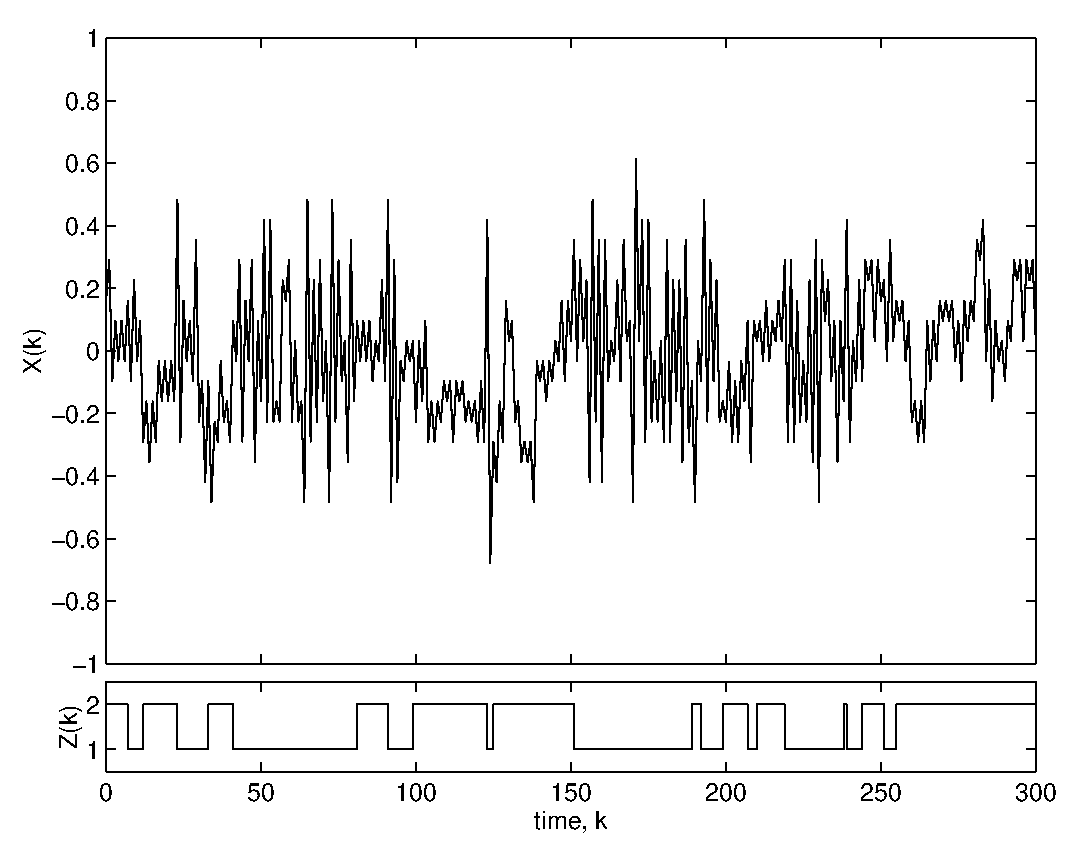
\includegraphics{fig/FigExTP1b_SamplePath.eps}}
  }
  \caption{\emph{The first 400 samples from a simulation of model B. The upper graph shows the turning points \emph{\texttt{x}} and the lower
    the regime process \emph{\texttt{z}}.}}
  \label{fig:SamplePathB}
\end{figure}

Next we calculate the rainflow matrices for the switching load, for
the subloads, and the superposition of the two subloads.
\begin{code}
>> GrfcB=smctp2rfm(P,{G1B,[];G2B,[]});
>> Grfc1B=mctp2rfm({G1B,[]});
>> Grfc2B=mctp2rfm({G2B,[]});
>> GrfcSumB=statP(1)*Grfc1B+statP(2)*Grfc2B;
\end{code}
Plot the matrices and compare \verb+GrfcB+ with \verb+GrfcSumB+.
What is your observations and conclusions?  Can you see the
switching when looking at the rainflow matrix?

%%%%%%%%%%%%%%%%%%%%%%%%%%%%%%%%%%%%%%%%%%%%%%%
% Observed Rainflow Matrix and Smoothing
%%%%%%%%%%%%%%%%%%%%%%%%%%%%%%%%%%%%%%%%%%%%%%%

\subsection{Observed Rainflow Matrix and Smoothing}

Now we consider model A again.
From the simulated load we can find the rainflow cycles and then
compute the observed rainflow matrix \verb+FrfcObs0+.
\begin{code}
>> TP = dat2tp([(1:T)' xD]);            % Turning points
>> RFC = tp2rfc(TP);                    % Rainflow cycles
>> paramD = [1 n n];
>> FrfcObs0 = cc2cmat(paramD,RFC);      % Observed rainflow matrix
\end{code}
For a discrete sequence of turning points (which \verb+xD+ is) one can
perform the above operation by one command
\begin{code}
>> FrfcObs = dtp2rfm(xD,n);             % Observed rainflow matrix
\end{code}
Compare the observed rainflow matrix \verb+FrfcObs+
%in Figure~\ref{fig1:rfcObs}a
with the theoretical one \verb+Grfc+.   %in Figure~\ref{fig1:rfc}c.
\begin{code}
>> cmatplot(u,u,{FrfcObs/(T/2) Grfc},1)
\end{code}

%\begin{figure}[htbp]
%  \centerline{
%  \begin{tabular}{cc}
%    {\small (a) Rainflow matrix, \texttt{FrfcObs}}   & {\small (b) Rainflow matrix, \texttt{FrfcSmooth}}  \\
%     \resizebox{\figwidthB}{!}{\includegraphics{fig/Fig1rfcObs.eps}} &
%    \resizebox{\figwidthB}{!}{\includegraphics{fig/Fig1rfcSmooth.eps}}
%  \end{tabular}
%  }
%  \caption{\emph{  (a) Observed rainflow matrix
%      \emph{\texttt{FrfcObs}} obtained from the simulation \emph{\texttt{x}}.
%      (b) \emph{\texttt{FrfcSmooth}} is obtained by smoothing \emph{\texttt{FrfcObs}}.  }}
%  \label{fig1:rfcObs}
%\end{figure}

If the observed rainflow matrix is too wiggly it can be smoothed
using \verb+smoothcmat+ to obtain a better estimate of the limiting
rainflow matrix. The smoothing procedure can also be used to
extrapolate (and interpolate) the observed rainflow matrix to cycles
that were not observed.
\begin{code}
>> h=0.8; FrfcSmooth = smoothcmat(FrfcObs,1,h);
>> cmatplot(u,u,{FrfcObs/(T/2) FrfcSmooth/(T/2) Grfc},1)
\end{code}
%Figure~\ref{fig1:rfcObs}b shows \verb+FrfcSmooth+ which has been
%obtained by smoothing \texttt{FrfcObs}.
The so called bandwidth
\verb+h+ is a smoothing parameter. Try different values of the
smoothing parameter \verb+h+ and see the difference.
A small \verb+h+ gives little smoothing, while a large \verb+h+ gives
much smoothing.

%%%%%%%%%%%%%%%%%%%%%%%%%%%%%%%%%%%%%%%%%%%%%%%
% Observed Rainflow Matrix and Smoothing
%%%%%%%%%%%%%%%%%%%%%%%%%%%%%%%%%%%%%%%%%%%%%%%

%\subsection{Extrapolation and Smoothing of Rainflow Matrices}
%
%To be added.

%%%%%%%%%%%%%%%%%%%%%%%%%%%%%%%%%%%%%%%%%%%%%%%
% Level Crossings
%%%%%%%%%%%%%%%%%%%%%%%%%%%%%%%%%%%%%%%%%%%%%%%

\subsection{Level Crossings}

Information about level crossings is contained in the rainflow
matrix.
\begin{code}
>> mu = cmat2lc(param,Grfc);
>> muSum = cmat2lc(param,GrfcSum);
>> muObs = cmat2lc(param,FrfcObs/(T/2));
>> subplot(2,1,1), plot(mu(:,1),mu(:,2),muSum(:,1),muSum(:,2),'--')
>> subplot(2,1,2), plot(mu(:,1),mu(:,2),muObs(:,1),muObs(:,2),'--')
\end{code}
%Figure~\ref{fig1:mu}a
The first plot compares the upcrossing intensity \verb+mu+ of
the switching load with the upcrossing intensity \verb+muSum+ of the
superimposed rainflow matrix.
Observe that, as expected, the switching gives rise
to more zero upcrossings than in the weighted sum of the individual
upcrossing intensities.
%In Fgure~\ref{fig1:mu}b
In the second plot the observed upcrossing intensity \verb+muObs+
is shown together with the theoretical one \verb+mu+.

%\begin{figure}[htbp]
%  \begin{tabular}{cc}
%    {\small (a) Crossing intensity} &
%    {\small (b) Crossing intensity} \\
%    \resizebox{\figwidthB}{!}{\includegraphics{fig/Fig1muSum.eps}} &
%    \resizebox{\figwidthB}{!}{\includegraphics{fig/Fig1muObs.eps}}
%  \end{tabular}
%  \caption{\emph{
%      (a) Level upcrossing intensity, \emph{\texttt{mu}} (--) compared
%      with the weighted sum \emph{\texttt{muSum}} (-- --).
%      (b) Level upcrossing intensity, \emph{\texttt{mu}} (--), compared with observed
%      upcrossing intensity \emph{\texttt{muObs}} (--) obtained from the
%      simulation \emph{\texttt{x}}.
%      }}
%  \label{fig1:mu}
%\end{figure}

%%%%%%%%%%%%%%%%%%%%%%%%%%%%%%%%%%%%%%%%%%%%%%%
% Damage
%%%%%%%%%%%%%%%%%%%%%%%%%%%%%%%%%%%%%%%%%%%%%%%

\subsection{Damage}

The toolbox contains routines for calculating the damage of a
load. The Palmgren-Miner damage hypothesis together with the W�hler
curve is used. This leads to the damage
\begin{equation}
  {\cal D}_{\beta} = \sum \frac{1}{N_{s_i}}
  = \sum K\left(S_i^{\rfc}\right)^{\beta}, \qquad
  S_i^{\rfc} = \left(M_i-m_i^{\rfc}\right)/2
\end{equation}
where $K$ and $\beta$ are material parameters. (The routines use
$K=1$.) The routines are  \verb+cc2dam+ for a cycle count (e.g.\
rainflow cycles) and
\verb+cmat2dam+ for a cycle matrix (e.g.\ rainflow matrix).
\begin{code}
>> beta = 4;
>> Dam = cmat2dam(param,Grfc,beta)
>> DamSum = cmat2dam(param,GrfcSum,beta)
>> DamObs = cc2dam(u(RFC),beta)/(T/2)
\end{code}
The calculated damages are scaled to damage per cycle, giving the results
\verb+Dam=0.0098+, \verb+DamSum=0.0017+ and for the simulation
\verb+DamObs=0.0097+. The damage from the simulation can also be
computed from \verb|FrfcObs| by using \verb|cmat2dam|.

The damage matrix is calculated by \verb+cmat2dmat+ and shows how the
damage is distributed among the different cycles. The sum of all the
elements in the damage matrix gives the total damage.
\begin{code}
>> Dmat = cmat2dmat(param,Grfc,beta);
>> DmatSum = cmat2dmat(param,GrfcSum,beta);
>> subplot(1,2,1), cmatplot(u,u,Dmat), axis('square'), v=axis;
>> subplot(1,2,2), cmatplot(u,u,DmatSum), axis('square'), axis(v)
\end{code}
Note that the rainflow matrix for the switching process gives much more
damage than that of the simple superposition.

%%%%%%%%%%%%%%%%%%%%%%%%%%%%%%%%%%%%%%%%%%%%%%%
% Decomposition of a Mixed rainflow matrix
%%%%%%%%%%%%%%%%%%%%%%%%%%%%%%%%%%%%%%%%%%%%%%%

\section{Decomposition of a Mixed Rainflow Matrix}
\label{lab2:Decomposition}

When collecting a load history, in the form of a rainflow matrix, all
the cycles of the switching load are stored in
one mixed rainflow matrix. Hence, there is a
need to interpret the mixed rainflow matrix, and e.g.\ tell how much
of the different load types a vehicle has experienced.

Here we will see that one can use the methods in \cite[Chapter~8]{Johannesson99.PhD} for decomposition of a mixed rainflow
matrix, i.e.\ methods for estimation of a SMCTP model given a
measurement of a mixed rainflow matrix.
Hence, the task is to estimate the
characteristics of the different subloads as well as the
characteristics of the switching between
the different subloads. The fact that we are able to
calculate the mixed expected rainflow matrix for a SMCTP model makes this estimation possible.
The principle of the decomposition is to find the best fit between the
measured rainflow matrix and the theoretically computed one, i.e.\ the
expected rainflow matrix. One problem is to decide what to mean by
``best fit''. The maximum likelihood (ML) method is often the best
method and yields the model that is ``the most probable one''. We will
propose an approximate ML estimator. There is also the
possibility to minimize the distance between the measured and the
theoretical rainflow matrices. We will propose three such distances,
namely the chi-square, the Hellinger, and the Kullback-Leibler distances.

\section{Model and Estimation}
\label{SecEst:ModelEstimation}

We want to estimate a SMCTP model, where the
number of regime states $r$ is fixed.
The model is parametrized by the min-max and the max-min transition
matrices
\begin{displaymath}
  \bm{Q}^{(1)},\ldots,\bm{Q}^{(r)}
  \qquad \mbox{and} \qquad
  \bmh{Q}^{(1)},\ldots,\bmh{Q}^{(r)}
\end{displaymath}
respectively,
and the transition matrix $\bm{P}$ for the regime process.

Obviously, one would like to estimate the whole model, i.e.\
%the number of subloads $r$,
the $\bm{P}$-matrix, and the subloads.
However, this is not possible, since the number of parameters in the
SMCTP model is larger than the number of observations, i.e.\ the
number of elements in the rainflow matrix.
Therefore, one
needs to impose some additional structure on the model in order to get fewer
parameters to estimate.

Sometimes the min-max matrices of the subprocesses
are known (or can be considered known) and thus the parameters of
the subloads are given.
Hence, in this case, only the transition matrix
$\bm{P}$ needs to be estimated.
For a SMCTP with two regime states we have a model with the parameters
\begin{displaymath}
  \bm{P}=\left(
    \begin{array}{cc}
      1-p_1 & p_1 \\
      p_2   & 1-p_2
    \end{array}
    \right),\quad
    \bm{Q}^{(1)},\bmh{Q}^{(1)},
    \bm{Q}^{(2)},\bmh{Q}^{(2)}
\end{displaymath}
and when the models of the subloads are known, then only the
parameters $\bm{\theta}=\left( p_1, p_2 \right)$ need to be estimated.
One such case is when the measured
rainflow matrix is believed to be a mixture of known standard
rainflow matrices, which could e.g.\ reflect different parts of a
testing track.
The goal is then to find the
proportion and the switching frequency of the different subprocesses.
All this information is contained in the $\bm{P}$ matrix.

Define a SMCTP model and simulate it in order to obtain an observed
mixed rainflow matrix.
\begin{code}
>> n = 8; param = [-1 1 n];
>> M1.x0=[-0.4 -0.3]; M1.s=0.15; M1.lam=1;
>> M2.x0=[0.3 0.4]; M2.s=0.15; M2.lam=1;
>> G1 = mktestmat(param,M1.x0,M1.s,M1.lam);
>> G2 = mktestmat(param,M2.x0,M2.s,M2.lam);
>> P=[1-0.1 0.1; 0.05 1-0.05]                % Transition matrix
>> [xD,z] = smctpsim(P,{G1 []; G2 []},5000); % Simulate
>> Fobs = dtp2rfm(xD,n);                     % observed mixed rainflow matrix
\end{code}
In order to get reasonably short computing times in Matlab when doing
the decomposition, we have chosen only 8 discrete levels.
However, the programs for doing the decomposition don't have any limitations in the size of the model.

\subsubsection*{Three Scenarios} \label{SecEst:Scenarios}

We will consider three cases of specifying the parameter vector $\bm{\theta}$, that we
want to estimate, depending on how much knowledge we have on the
min-max matrices. The approximate ML method will be used.
\begin{enumerate}
\item The min-max matrices of the subloads can be considered known, so
  that only the regime process is unknown, and only the parameters
  $p_1$ and $p_2$ need to be estimated.
  $\bm{\theta}=(p_1,~p_2)$
\begin{code}
>> known1.F = {G1 []; G2 []}; % known min-max and max-min matrices
>> init1.P = P;               % initial guess of P-matrix
>> [Fest1,Est1] = estsmctp(Fobs,'P','ML',known1,[],init1);
>> Est1.P                     % Estimated P-matrix
\end{code}
\item Here the  min-max matrix for each subload $z$ is
  specified, but we allow a translation $\tilde{m}_z$ and a scaling $\tilde{s}_z$,
  which are used
  as parameters for the subloads. The translation $\tilde{m}_z$ corresponds to a change of the mean
  level and the scaling $\tilde{s}_z$ corresponds to a change in the variance for the subload,
  i.e.\ a transformation of the form
  $X^{(z)}(t)=\tilde{s}_z \tilde{X}^{(z)}(t) + \tilde{m}_z$,
  where $\tilde{X}^{(z)}(t)$ is the process according to the specified
  min-max matrix.
  Now we have six parameters to estimate,\\
  $\bm{\theta}=(p_1,~p_2,~\tilde{m}_1,~\tilde{s}_1,~\tilde{m}_2,~\tilde{s}_2).$
\begin{code}
... Estimate ...
\end{code}
\item Here we will use, for each subload, the parametric model
  described by Eqs.~(8.15,8.16) with four
  parameters. In total this gives ten parameters to estimate,\\
  $\bm{\theta}=(p_1,~p_2,~x_{11}~,x_{21}~,s_1~,\lambda_1,~x_{12}~,x_{22}~,s_2~,\lambda_2)$.
\begin{code}
>> known3.Ffun = 'f_funm';   % Function for calculating a submodel
>> known3.trModel2X = 'tr_m2x'; % transform from Model to X-vector
>> known3.trX2Model = 'tr_x2m'; % transform from X-vector to model
>> known3.param =param;
>> init3.P = P;              % initial guess of P-matrix
>> init3.M = {M1 M2};        % initial guess of Models for min-max mat
>> [Fest3,Est3] = estsmctp(Fobs,'P,CalcF','ML',known3,[],init3);
>> Est3.P                    % Estimated P-matrix
>> Est3.M{:}                 % Estimated parameters in models
\end{code}
\end{enumerate}

\subsubsection*{Estimation from a Measurement of the Regime Process}

If the regime process $\{Z_k\}$ itself is observed, then one has as much
information about the switching that one can possibly get.
The ML estimates of $p_1$ and
$p_2$ can easily be obtained from the observed regime process,
$\bm{z}=\{z_k\}_{k=0}^T$, see \cite[Appendix~A]{Johannesson99.PhD}.
%This estimator
%will be denoted ML-z, and will serve as our reference
%estimator, as no other estimator can perform better than ML-z, by
%means of bias and variance. We will be happy if the performance of some other method
%is almost as good as ML-z.
\begin{code}
>> Pest_z = estmc(z,2)
\end{code}

Compare the estimated stationary distributions and the true one:
\begin{code}
>> mc2stat(Est1.P)
>> mc2stat(Est3.P)
>> mc2stat(Pest_z)
>> mc2stat(P)
\end{code}

\subsection*{Methods for Estimation (Optional)}

The four methods for estimation, described in
\cite[Section~8.2]{Johannesson99.PhD}, will now be examined. The first
method is the approximate maximum
likelihood (AML) estimator, where we assume that the sample of the
rainflow matrix is a sample from a multinomial distribution.
The next three methods are based on minimizing the
distance between the measured rainflow matrix and the expected
rainflow matrix. The distances that will be used are, the
chi-square distance ($\chi^2$), the Hellinger distance (HD), and the
Kullback-Leibler distance (KL).
The estimates are obtained by numerical optimization by using the
routine \verb+fmins+, see
\cite[Section~8.6]{Johannesson99.PhD} for further details.
\begin{code}
>> known.F = {G1 []; G2 []};   % known min-max and max-min matrices
>> init.P = P;                 % initial guess of P-matrix
>> [Fest,Est] = estsmctp(Fobs,'P','ML',known,[],init); Est.P
>> [Fest,Est] = estsmctp(Fobs,'P','chi2',known,[],init); Est.P
>> [Fest,Est] = estsmctp(Fobs,'P','HD',known,[],init); Est.P
>> [Fest,Est] = estsmctp(Fobs,'P','KL',known,[],init); Est.P
\end{code}
